% !TeX root = ../main.tex

\section*{Manifold Learning}
Pricipal idea: Reduce the dimensions of the Data, gut preserve the sturcture of the data / underling manifold.

\subsection*{Curse of Dimensionality}
``Human intuition breaks in high dimensional spaces :(''

\paragraph{Let's illustrate this:}
Consider a d-dimensional feature vector $\vec{x_1}, \vec{x_2}, \dots, \vec{x_N} \in \mathbb{R}^d$ where $0 \le x_{i,k} \le 1$ (??? wo kommt das k her) uniformly distributed in a d-dimensional hyperspace of volume 1.
Let's say we would like to cover enough volume of  the cube to collect $1\%$ of the data. Let's say we also use a cube for this task. What is the required edge length $s$ of the cube to obtain that $1\%$ of space?

\paragraph{Example:}
A 10 dimensional hypercube

\begin{equation*}
    V=s^d \Rightarrow s = V^{\frac{1}{d}} = 0,01^{\frac{1}{10}} = 0.63
\end{equation*}

\begin{figure}[H]
	\centering
	
\includegraphics[width=0.5\textwidth]{todo}
\end{figure}

Another way of thinking about this is, that in a very high dimensional space, virtually every feature point is located at the boudary of the feature space\footnote{Because in at least on dimension, we draw a very low of very high value}. This leads to the effect, that common distance measues loose their  effectivity. E.g. the \textit{median} distance fo the nearest neighbour to the origin.

\subsection*{Techniques for dimensionality reduction}


\subsection*{Multi Dimensional Scaling (MDS)}
\subsection*{ISOMAP Algorithm}
\subsection*{Locally Linear Embedding (LLE)}
\subsection*{Laplacian Eigenmaps}
\subsection*{Random Forrest}


% \paragraph{Variants of k-means:}
% For clustering see section 14 of ``The Elements of Statistical Learning'' (Hastie, Tibshirani, Friedman - 2009). Section 14.3 ``Cluster Analysis'' introduces different flavours of k-means. Points of interest are:
% \begin{itemize}
% 	\item Proximity Matrices
% 	\item K-means
% 	\item Gaussian Mixtures as Soft K-means Clustering
% 	\item Vector Quantization
% \end{itemize}
%
% \paragraph{Q:} How can we determine k?
%
% Let $w(c)$ be distance from samples to cluster centres within clusters. We use this as a metric of quality in cluster analysis.
%
% \subparagraph{Approach 1:} Track the rate of change of a quality metric (like $w(c)$). Proposed in ``Pattern Classification'' (Duda, Hart, Stork).
%
% \begin{figure}[H]
% 	\centering
% 	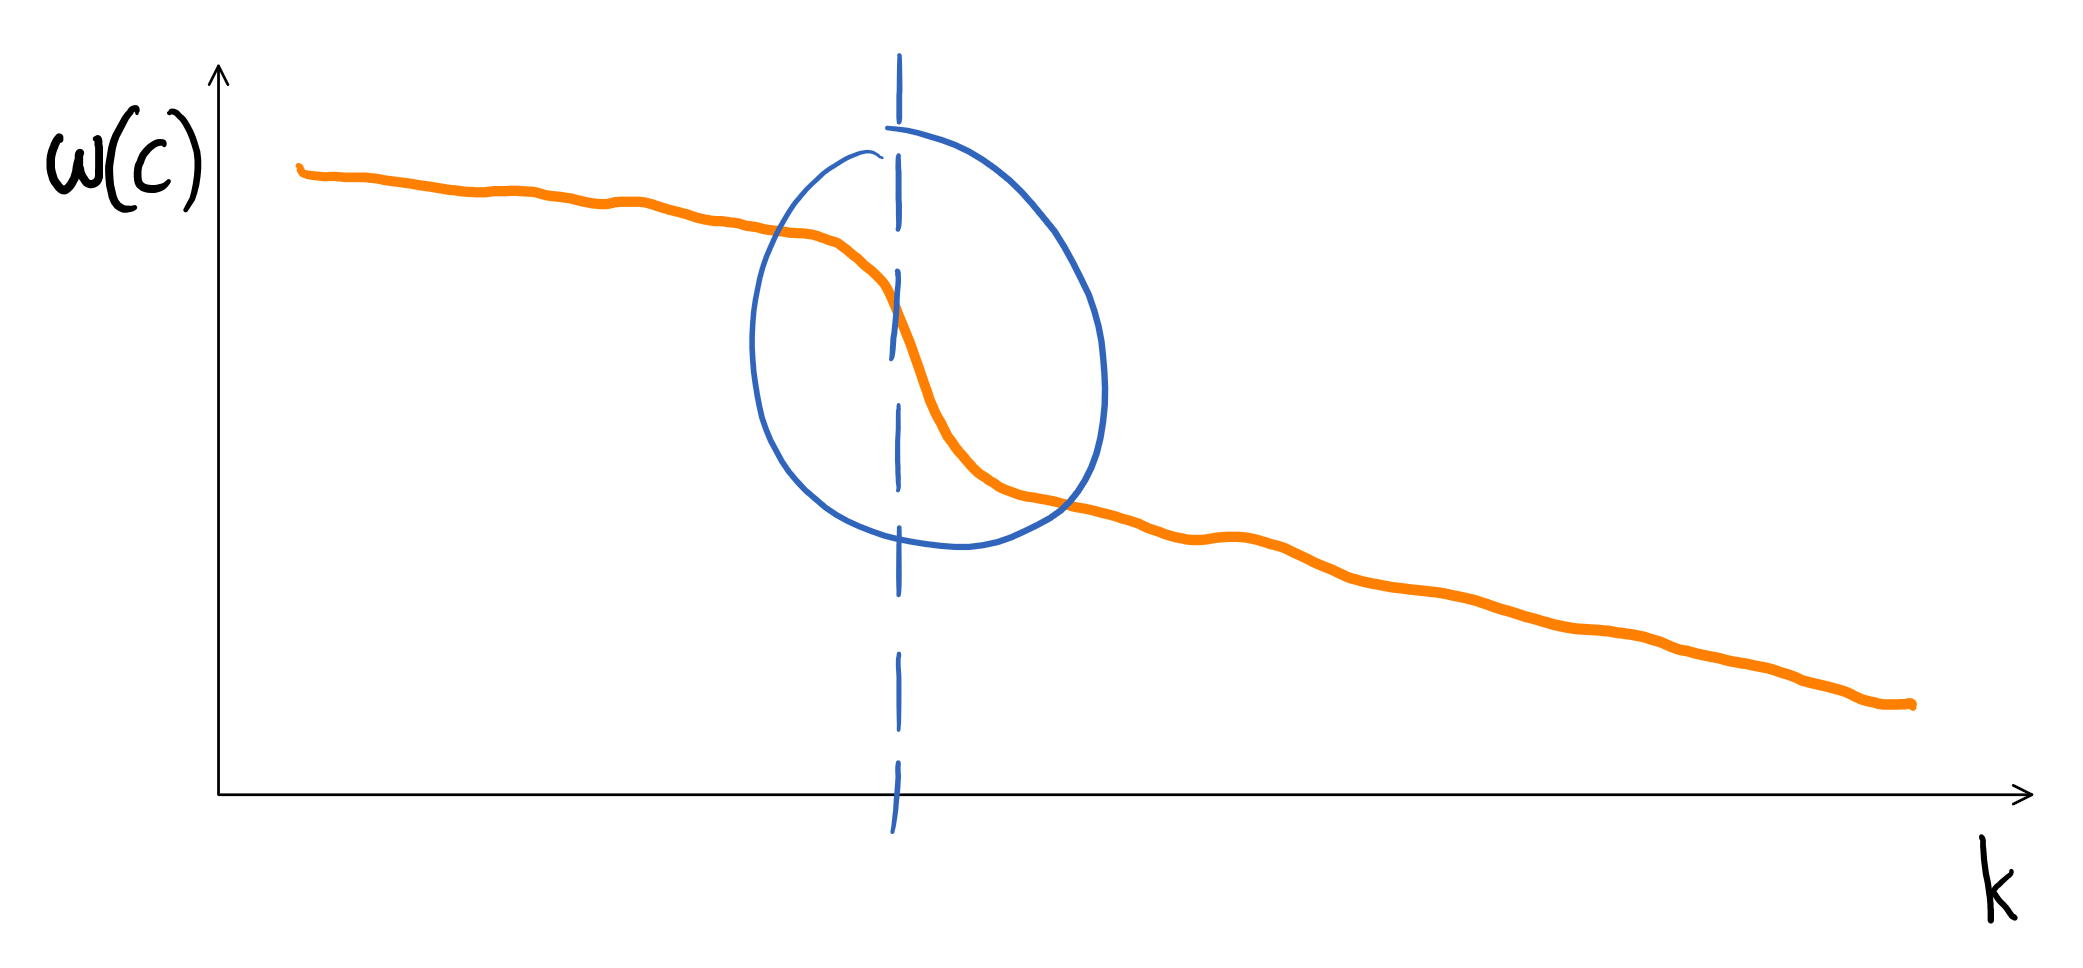
\includegraphics[width=0.8\textwidth]{07-rate-of-change}
% \end{figure}
%
% \subparagraph{Approach 2:} Let $w'(c)$ be a metric on a uniform distribution of samples. Relate change of $w(c)$ to change of $w'(c)$. Proposed in TEoSL.
%
% \begin{figure}[H]
% 	\centering
% 	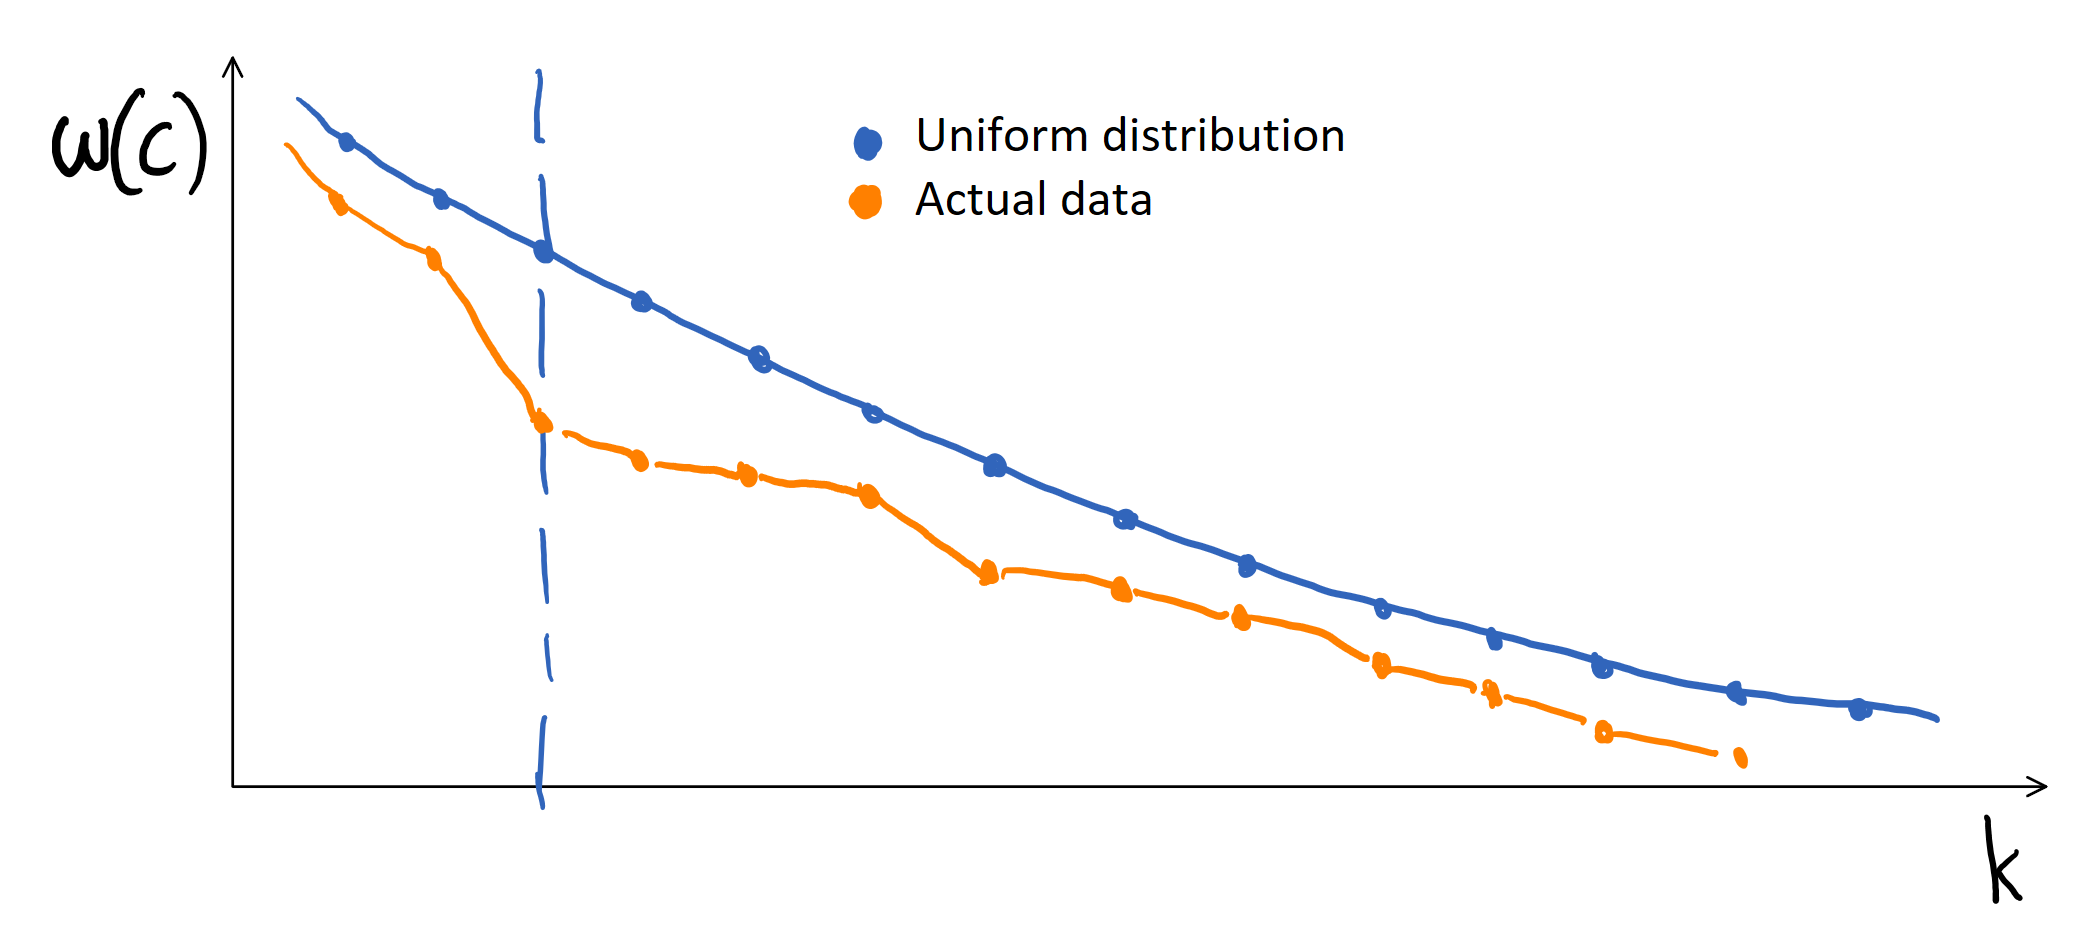
\includegraphics[width=0.8\textwidth]{08-w_c-vs-w_prime_c}
% \end{figure}
